
\documentclass[manuscript,screen,review]{acmart}
\usepackage{graphicx}
\usepackage{subcaption}
\usepackage{todonotes}
\usepackage{hyperref}


\AtBeginDocument{%
  \providecommand\BibTeX{{%
    \normalfont B\kern-0.5em{\scshape i\kern-0.25em b}\kern-0.8em\TeX}}}



%% These commands are for a PROCEEDINGS abstract or paper.
\acmConference[Conference acronym 'XX]{Make sure to enter the correct
  conference title from your rights confirmation emai}{June 03--05,
  2018}{Woodstock, NY}


\acmBooktitle{Woodstock '18: ACM Symposium on Neural Gaze Detection,
 June 03--05, 2018, Woodstock, NY} 



\begin{document}

%%
%% The "title" command has an optional parameter,
%% allowing the author to define a "short title" to be used in page headers.
\title[Analyse von neuronal networks und climate change temperature data]{Analyse von neuronal network Architekturen im Bezug auf climate change temperature data}

%%
%% The "author" command and its associated commands are used to define
%% the authors and their affiliations.
%% Of note is the shared affiliation of the first two authors, and the
%% "authornote" and "authornotemark" commands
%% used to denote shared contribution to the research.
\author{Torge Schwark}
\authornote{Both authors contributed equally to this research.}
\email{stuTODO:@mail.uni-kiel.de}
\orcid{1234-5678-9012}
\author{Joschua Quotschalla}
\authornotemark[1]
\email{stu235352@mail.uni-kiel.de}
\affiliation{%
  \institution{Institute of Computer Science, University of Kiel}
  \streetaddress{P.O. Box 1212}
  \city{Kiel}
  \state{Schleswig-Holstein}
  \country{Germany}
  \postcode{2411TODO:}
}



\keywords{neuronale Netzwerke, NN, MLP, 1D CONV, LSTM, Transformer, Klimawandel, Temperatur}


\maketitle


\section{Einleitung}
Der Klimawandel ist zweifellos eine der größten Herausforderungen unserer Zeit, und die präzise Vorhersage von klimatischen Veränderungen wird zunehmend unerlässlich. In diesem Kontext konzentriert sich diese Forschung darauf, leistungsfähige Neuronale Netze zu trainieren, um nicht nur bestehende Vorhersagen zu verbessern, sondern auch entscheidende Erkenntnisse über die zukünftige Entwicklung unserer Umwelt zu gewinnen.

\subsection{Verwendeter Datensatz und Untersuchte Modelle}
Die Grundlage dieser Forschung bildet der Datensatz "Climate Change: Earth Surface Temperature Data". Durch die Analyse und Anwendung verschiedenster Architekturen von MLPs, LSTMs, ConvNets und Transformern wurden Neuronale Netze trainiert, um bestmögliche Vorhersagen für künftige Klimaentwicklungen zu erzielen. Die Vielfalt der Modelle ermöglicht nicht nur eine gründliche Untersuchung ihrer Leistungsfähigkeit, sondern auch die Identifikation der optimalen Architektur für präzise Klimavorhersagen.

\subsection{Schwerpunkt: Das Training Neuronaler Netze}
 Durch eine Abstimmung von Modellarchitekturen mit den Hyperparametern wird sichergestellt, dass die trainierten Neuronalen Netze nicht nur auf bereits existierende Daten gut abgestimmt sind, sondern auch eine überzeugende Präzision in der Vorhersage von langfristigen Klimaveränderungen aufweisen. 

\subsection{Ziel des Trainings}
Unser Ziel besteht darin, fundierte Klimavorhersagen für die kommenden 100 Jahre zu treffen und gleichzeitig einen tiefgreifenden Einblick in die globalen Temperaturtrends zu gewinnen. Dies ermöglicht nicht nur eine bessere Anpassung an den Klimawandel, sondern auch die Entwicklung effektiver Strategien zur Bewältigung seiner Auswirkungen.


\section{Methoden}
\subsection*{Datensatz und Datenaufbereitung}
\begin{itemize}
    \item Umfassende Analyse des Datensatzes: Histogramme, Barcharts, Landkarten.
    \item Überprüfung auf Duplikate, insbesondere gleiche Städte.
    \item Aufteilung in Trainings- und Validierungssets (70/30).
    \item Filterung von Zeiträumen mit konstanten Daten über 95 Jahre.
\end{itemize}

\subsection*{Training der Neuronalen Netze}
\begin{itemize}
    \item Berechnung des MAE über 720 menschliche Vorhersagen als Bezugsgröße.
    \item Anwendung einer Grid Search-Methode für MLPs, ConvNets, LSTMs.
    \item Feintuning: Anpassung von Hyperparametern, Augmentation, Normalisierung.
\end{itemize}

\subsection*{Auswertung}
\begin{itemize}
    \item Prüfen auf Overfitting, Analyse des Loss Graphen.
    \item Vergleich des MAE mit menschlichen Vorhersagen.
    \item Analyse der Genauigkeit an Beispielen.
\end{itemize}

\subsection*{Anwendung}
\begin{itemize}
    \item Anwendung des besten Netzwerks für Vorhersagen bis 2100.
    \item Erstellung eines Durchschnittsgraphen von 1750 bis 2100.
\end{itemize}



\section{Datensatz}
\subsection{Einführung und Datenverständnis}
Die Grundlage dieser Studie bildet der \href{https://www.kaggle.com/datasets/berkeleyearth/climate-change-earth-surface-temperature-data?select=GlobalLandTemperaturesByCity.csv}{"Climate Change: Earth Surface Temperature"} Datensatz.
Der genannte Datensatz umfasst insgesamt 10.064.718 monatliche Durchschnittstemperaturen, die in 3.448 Städten und 159 Ländern erhoben wurden. Die Aufzeichnungen reichen dabei von den frühesten Daten im Jahr 1743 bis zu den aktuellsten im Jahr 2015.

\subsection{Fehlende Daten und Ungenauigkeiten}
Bei unserer Analyse auf Duplikate stellten wir fest, dass sich 117 Städte im Datensatz doppelt oder mehrfach vorkommen. Diese doppelten Einträge sind vermutlich auf die Tatsache zurückzuführen, dass der Datensatz eine Zusammenstellung von 16 bereits bestehenden Datenarchiven darstellt.
Zusätzlich zu den Duplikaten ist zu berücksichtigen, dass Temperaturmessungen, keine exakten Werte liefern. Daher sind im Datensatz zu den jeweiligen durchschnittlichen Temperaturen auch die durchschnittlichen Messunsicherheiten aufgeführt. Obwohl diese Unsicherheiten stetig abnehmen, stellen sie dennoch eine Herausforderung für die Vorhersagegenauigkeit dar. Bei der Betrachtung der Messungenauigkeit ist jedoch zu beachten, dass der exakte Messwert mit hoher Wahrscheinlichkeit eine geringere Abweichung aufweist als die Messunsicherheit. Daher ist der durchschnittliche Messfehler deutlich geringer als die Messunsicherheit.
Besonders in den frühen Jahren der Temperaturaufzeichnung sind zudem Monate vorhanden, für die keine Werte protokolliert wurden.

\subsection{Data-Loader Pipeline}
Die Data-Loader Pipeline wurde implementiert, um Mini-Batches von Sequenzen von Datenpunkten gemäß den Anforderungen der Architekturen bereitzustellen. Dabei musste sichergestellt werden, dass Datenpunkte für die gesammte input länge von 70 Jahren(840 Monaten) und output länge von 25 Jahren(320 Monate) ohne Lücken vorhanden sind.
Um die Effizienz des Trainings zu steigern, erfolgte die Extraktion der Daten aus den fünf CSV-Dateien, wobei für jeden Standort eine eigene Textdatei angelegt wurde. Zu Beginn wählten wir einen zufälligen Standort und einen zufälligen Zeitraum in dem 90 Jahre vollstänige Messwerte vohanden waren.
Später versuchten wir den Data-Loader weiter zu verbessern, dazu speicherten wir die gesamten Daten zunächst in Listen und führten die Suche nach passenden Zeiträumen einmalig am Anfang des Trainings durch. Diese Optimierung brachte jedoch nicht den gewünschten Effekt.

Die spätere Anwendung von Multiprocessing zur Ausführung des Data-Loaders auf bis zu 20 Prozessen gleichzeitig beschleunigte den Data-Loader mit minimalem Aufwand um etwa das Zehnfache und erhöhte die Hardware-Auslastung merklich. Der Flaschenhals lag dabei im Arbeitsspeicher.

\subsection{Visualisierungen für Datenanalyse und Predictions}
\begin{figure}[htp]
  \centering
  \begin{subfigure}{.45\textwidth}
      \centering
      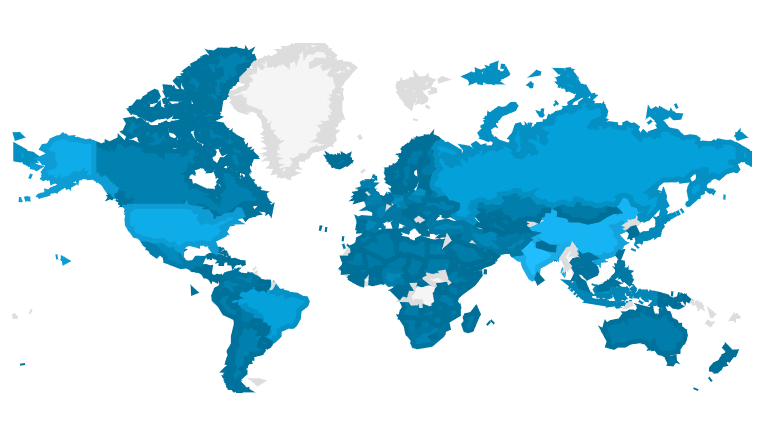
\includegraphics[width=.8\linewidth]{./histograms/map_plot_data_points}
      \caption{Histogram}
      \label{fig:sub1}
  \end{subfigure}%
  \begin{subfigure}{.45\textwidth}
      \centering
      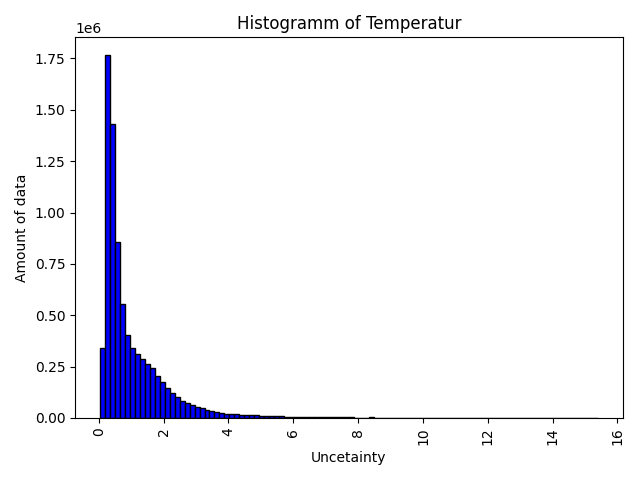
\includegraphics[width=.8\linewidth]{./histograms/Uncertainty}
      \caption{Histogram 2}
      \label{fig:sub2}
  \end{subfigure}\\
  \begin{subfigure}{.45\textwidth}
      \centering
      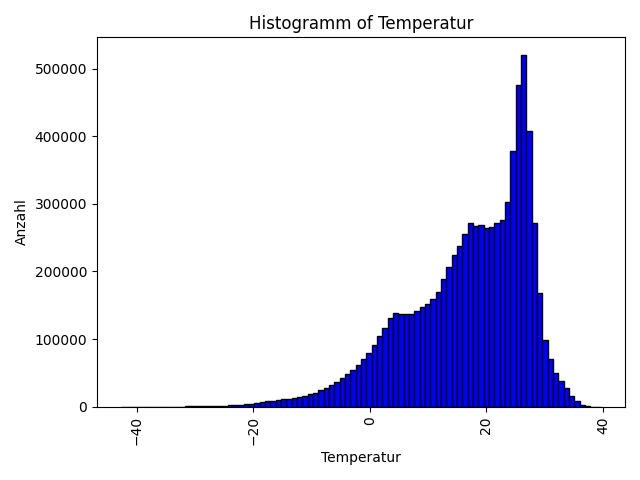
\includegraphics[width=.8\linewidth]{./histograms/Temperatur}
      \caption{Histogram 3}
      \label{fig:sub3}
  \end{subfigure}%
  \begin{subfigure}{.45\textwidth}
      \centering
      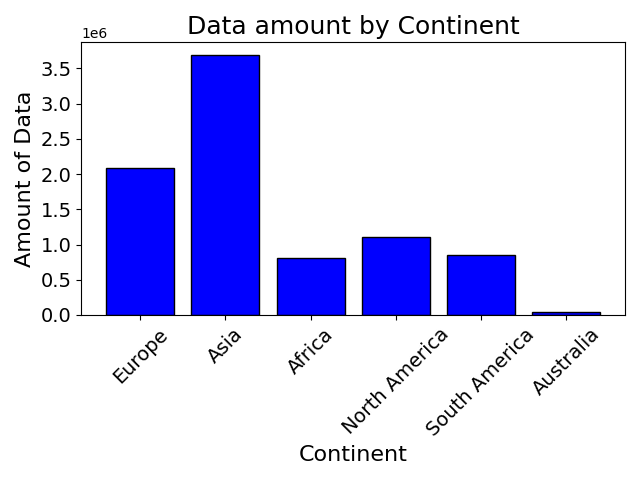
\includegraphics[width=.8\linewidth]{./histograms/Continents}
      \caption{Histogram 4}
      \label{fig:sub4}
  \end{subfigure}
  \caption{Four histograms}
  \label{fig:test}
  \Description{Histograms caputuring the distribution of the data.}
\end{figure}

Für die Analyse wurden Visualisierungen wie Histogramme für geografische Merkmale, Datenverteilungen und Kartenplots verwendet. T-SNE-Plots ermöglichten eine multidimensionale Darstellung der Datenpunkte für eine verbesserte Analyse.



\section{Training-Procedure}

\begin{table}
  \caption{Network Architekturen}
  \label{tab:freq}
  \begin{tabular}{ccl}
    \toprule
    Netzwerk&Anzahl Parameter&Anzahl Layern\\
    \midrule
    MLP & TODO: & meisten Parameter aufgrund von dense layern\\
    CONV 1D & TODO: & geringere Anzahl durch feature extraction convolution layer vor den dense layern\\
    LSTM & TODO: & TODO:\\
    Transformer & TODO: & (zweit) meisten Parameter aufgrund von mehreren inneren MLPs\\
  \bottomrule
\end{tabular}
\end{table}

Die Netzwerkarchitekturen MLP, 1D Conv Net, LSTM und Transformer wurden auf den vorbereiteten Datensätzen trainiert. 
Im ersten Schritt wurde eine Grid Search durchgeführt, um die optimalen Modelle und deren Hyperparameter zu bestimmen. 
Nach dieser automatisierten Suchstrategie wurde ein händisches Fine-Tuning durchgeführt, um die Leistung der Modelle weiter zu verbessern. 
Während des gesamten Prozesses wurde darauf geachtet, wie sich jede Architektur an die spezifischen Charakteristiken des Datensatzes anpasst und 
wie gut sie die Temperaturvorhersagen durchführen kann. 
Die sorgfältige Auswahl und Anpassung der Hyperparameter und Aktivierungsfunktionen spielte eine entscheidende Rolle bei der Optimierung der Modellleistung.

Rewe GPT:
Optimierung von Architekturen und Parametern
Die Auswahl und Optimierung der geeigneten Parameter für neuronale Netzwerkarchitekturen spielt eine entscheidende Rolle bei der Leistungsfähigkeit und Zuverlässigkeit der Klimavorhersagemodelle. 
Im Rahmen der Untersuchung wurden verschiedene Schlüsselparameter betrachtet und optimiert, um die bestmöglichen Ergebnisse zu erzielen.

\textbf{MLP (Multilayer-Perzeptronen)}
Im Kontext von Multilayer-Perzeptronen (MLPs) spielen insbesondere die Anzahl der Hidden Layers, die Anzahl der Neuronen pro Layer, 
die Wahl der Aktivierungsfunktionen und die Lernrate eine bedeutsame Rolle bei der Optimierung. 
Die Anpassung dieser Parameter beeinflusst maßgeblich die Fähigkeit des MLP-Modells, komplexe nichtlineare Zusammenhänge zu erfassen und präzise Vorhersagen zu generieren. 
Unsere Experimente haben gezeigt, dass die Auswahl und Feinabstimmung dieser Parameter entscheidend sind, um eine ausgewogene Modellkapazität zu gewährleisten und \textcolor{gray}{Überanpassung/Overfitting} zu vermeiden.
Die systematische Optimierung der genannten Architekturen und Parameter bildet die Grundlage für die Evaluierung ihrer Leistungsfähigkeit im Kontext der Klimavorhersage. 
Es ist wichtig, die spezifischen Verhaltensweisen und Interaktionen der Optimierungsergebnisse zu analysieren, um fundierte Schlussfolgerungen hinsichtlich der Vorhersagequalität und der Quantifizierung des Modellverhaltens ziehen zu können.

\textbf{LSTMs (Long Short-Term Memory Networks)}
Ein zentraler Parameter bei LSTMs ist die Anzahl der Memory Units oder sogenannten Neuronen in der Zelle. Durch gezielte Anpassung dieser Anzahl kann die Netzwerkleistung verbessert 
und die Fähigkeit zur Erfassung von langfristigen Abhängigkeiten gesteuert werden. 
In dem Experimenten wurde festgestellt, dass eine moderate Anzahl von Memory Units zu einer ausgewogenen Leistung führt, während zu wenige Units die Kapazität des Netzwerks begrenzen und zu schlechterer Modellleistung führen können.

\textbf{Convolutional Neural Networks (ConvNets)}
Für ConvNets sind insbesondere die Größe und Anordnung der \textcolor{gray}{Kernel/Filter} sowie deren Anzahl in den Convolutional Layern von großer Bedeutung. 
Während größere \textcolor{gray}{Kernel/Filter} und eine höhere Anzahl von Filtern zu einer komplexeren Modellarchitektur und möglicherweise zu einer besseren Erfassung räumlicher Merkmale führen können, 
besteht die Herausforderung darin, ein ausgewogenes Verhältnis zu finden, das Overfitting vermeidet und effektivere Modelle ermöglicht.

\textbf{Transformer-Architekturen}
Bei der Optimierung von Transformer-Modellen, insbesondere in Bezug auf Klimavorhersagen, sind die Anzahl der Layer, die Dimensionalität der Embeddings, die Anzahl der Köpfe in den Multi-Head Attention Mechanismen und die Lernrate wichtige Parameter. Unsere Untersuchungen haben gezeigt, dass die sorgfältige Abstimmung dieser Parameter in einem komplexen Zusammenspiel entscheidend ist, um eine optimale Leistungsfähigkeit der Transformer-Architekturen zu erreichen.
Es ist wichtig zu betonen, dass Optimierungsansätze stark von den spezifischen Merkmalen des betrachteten Datensatzes und den Zielsetzungen der Klimavorhersagen abhängen. Daher ist eine systematische und gewissenhafte Evaluierung der Optimierungsergebnisse unerlässlich, um fundierte Schlussfolgerungen hinsichtlich der Performanz der unterschiedlichen Architekturen zu ziehen.


\subsection{Architekturvergleich und Normalisierungen}

Die Leistung der Architekturen wurde sowohl qualitativ als auch quantitativ bewertet. Aktivierungsfunktionen wie Selu und Relu wurden für MLP analysiert. Bei 1D Conv Net wurde die Auswirkung von Global Average Pooling und Flatten vor den Dense Layern untersucht. LSTM und Transformer wurden auf ihre spezifischen Eigenschaften und Fehlerquellen analysiert. Der Vergleich erfolgte durch Bewertung der qualitativen Anpassung und quantitativen Metriken wie dem Mean Absolute Error (MAE).


\subsection{Normalisierung und Variation der Input-Sequenzen}

Die Daten wurden vor dem Training normalisiert, und die Auswirkungen auf die Vorhersagegenauigkeit wurden verglichen. Zusätzlich wurde die Performance der Modelle für variable Input-Sequenzen von 8, 16, 32 und 64 untersucht. Dies ermöglichte eine tiefgreifende Analyse, wie die Länge der Input-Sequenzen die Modellleistung beeinflusst.


Insgesamt bietet diese Studie eine umfassende Analyse der Climate Change-Daten unter Verwendung verschiedener Netzwerkarchitekturen. Die gewonnenen Erkenntnisse ermöglichen nicht nur eine bessere Anpassung der Modelle an die Daten, sondern auch Optimierungsmöglichkeiten für zukünftige Forschungen im Bereich des Klimawandels.

\section{Results}
\todo[size=\small]{TODO}

\section{Conclusion}
\todo[size=\small]{TODO}

\section{Citations and Bibliographies}

The use of \BibTeX\ for the preparation and formatting of one's
references is strongly recommended. Authors' names should be complete
--- use full first names (``Donald E. Knuth'') not initials
(``D. E. Knuth'') --- and the salient identifying features of a
reference should be included: title, year, volume, number, pages,
article DOI, etc.

The bibliography is included in your source document with these two
commands, placed just before the \verb|\end{document}| command:
\begin{verbatim}
  \bibliographystyle{ACM-Reference-Format}
  \bibliography{bibfile}
\end{verbatim}
where ``\verb|bibfile|'' is the name, without the ``\verb|.bib|''
suffix, of the \BibTeX\ file.

Citations and references are numbered by default. A small number of
ACM publications have citations and references formatted in the
``author year'' style; for these exceptions, please include this
command in the {\bfseries preamble} (before the command
``\verb|\begin{document}|'') of your \LaTeX\ source:
\begin{verbatim}
  \citestyle{acmauthoryear}
\end{verbatim}

  Some examples.  A paginated journal article \cite{Abril07}, an
  enumerated journal article \cite{Cohen07}, a reference to an entire
  issue \cite{JCohen96}, a monograph (whole book) \cite{Kosiur01}, a
  monograph/whole book in a series (see 2a in spec. document)
  \cite{Harel79}, a divisible-book such as an anthology or compilation
  \cite{Editor00} followed by the same example, however we only output
  the series if the volume number is given \cite{Editor00a} (so
  Editor00a's series should NOT be present since it has no vol. no.),
  a chapter in a divisible book \cite{Spector90}, a chapter in a
  divisible book in a series \cite{Douglass98}, a multi-volume work as
  book \cite{Knuth97}, a couple of articles in a proceedings (of a
  conference, symposium, workshop for example) (paginated proceedings
  article) \cite{Andler79, Hagerup1993}, a proceedings article with
  all possible elements \cite{Smith10}, an example of an enumerated
  proceedings article \cite{VanGundy07}, an informally published work
  \cite{Harel78}, a couple of preprints \cite{Bornmann2019,
    AnzarootPBM14}, a doctoral dissertation \cite{Clarkson85}, a
  master's thesis: \cite{anisi03}, an online document / world wide web
  resource \cite{Thornburg01, Ablamowicz07, Poker06}, a video game
  (Case 1) \cite{Obama08} and (Case 2) \cite{Novak03} and \cite{Lee05}
  and (Case 3) a patent \cite{JoeScientist001}, work accepted for
  publication \cite{rous08}, 'YYYYb'-test for prolific author
  \cite{SaeediMEJ10} and \cite{SaeediJETC10}. Other cites might
  contain 'duplicate' DOI and URLs (some SIAM articles)
  \cite{Kirschmer:2010:AEI:1958016.1958018}. Boris / Barbara Beeton:
  multi-volume works as books \cite{MR781536} and \cite{MR781537}. A
  couple of citations with DOIs:
  \cite{2004:ITE:1009386.1010128,Kirschmer:2010:AEI:1958016.1958018}. Online
  citations: \cite{TUGInstmem, Thornburg01, CTANacmart}. Artifacts:
  \cite{R} and \cite{UMassCitations}.





\section{SIGCHI Extended Abstracts}

The ``\verb|sigchi-a|'' template style (available only in \LaTeX\ and
not in Word) produces a landscape-orientation formatted article, with
a wide left margin. Three environments are available for use with the
``\verb|sigchi-a|'' template style, and produce formatted output in
the margin:
\begin{itemize}
\item {\verb|sidebar|}:  Place formatted text in the margin.
\item {\verb|marginfigure|}: Place a figure in the margin.
\item {\verb|margintable|}: Place a table in the margin.
\end{itemize}

%%
%% The acknowledgments section is defined using the "acks" environment
%% (and NOT an unnumbered section). This ensures the proper
%% identification of the section in the article metadata, and the
%% consistent spelling of the heading.
\begin{acks}
To Robert, for the bagels and explaining CMYK and color spaces.
\end{acks}

%%
%% The next two lines define the bibliography style to be used, and
%% the bibliography file.
\bibliographystyle{ACM-Reference-Format}
\bibliography{sample-base}

%%
%% If your work has an appendix, this is the place to put it.
\appendix


\section{Online Resources}

Nam id fermentum dui. Suspendisse sagittis tortor a nulla mollis, in
pulvinar ex pretium. Sed interdum orci quis metus euismod, et sagittis
enim maximus. Vestibulum gravida massa ut felis suscipit
congue. Quisque mattis elit a risus ultrices commodo venenatis eget
dui. Etiam sagittis eleifend elementum.

Nam interdum magna at lectus dignissim, ac dignissim lorem
rhoncus. Maecenas eu arcu ac neque placerat aliquam. Nunc pulvinar
massa et mattis lacinia.

\end{document}
\endinput
%%
%% End of file `sample-authordraft.tex'.